% Options for packages loaded elsewhere
\PassOptionsToPackage{unicode}{hyperref}
\PassOptionsToPackage{hyphens}{url}
%
\documentclass[
  14pt,
]{extarticle}
\usepackage{amsmath,amssymb}
\usepackage{lmodern}
\usepackage{iftex}
\ifPDFTeX
  \usepackage[T1]{fontenc}
  \usepackage[utf8]{inputenc}
  \usepackage{textcomp} % provide euro and other symbols
\else % if luatex or xetex
  \usepackage{unicode-math}
  \defaultfontfeatures{Scale=MatchLowercase}
  \defaultfontfeatures[\rmfamily]{Ligatures=TeX,Scale=1}
\fi
% Use upquote if available, for straight quotes in verbatim environments
\IfFileExists{upquote.sty}{\usepackage{upquote}}{}
\IfFileExists{microtype.sty}{% use microtype if available
  \usepackage[]{microtype}
  \UseMicrotypeSet[protrusion]{basicmath} % disable protrusion for tt fonts
}{}
\makeatletter
\@ifundefined{KOMAClassName}{% if non-KOMA class
  \IfFileExists{parskip.sty}{%
    \usepackage{parskip}
  }{% else
    \setlength{\parindent}{0pt}
    \setlength{\parskip}{6pt plus 2pt minus 1pt}}
}{% if KOMA class
  \KOMAoptions{parskip=half}}
\makeatother
\usepackage{xcolor}
\usepackage[margin=1.5cm,bottom=2.5cm,top=2.5cm,headsep=0cm,headheight=5cm]{geometry}
\usepackage{graphicx}
\makeatletter
\def\maxwidth{\ifdim\Gin@nat@width>\linewidth\linewidth\else\Gin@nat@width\fi}
\def\maxheight{\ifdim\Gin@nat@height>\textheight\textheight\else\Gin@nat@height\fi}
\makeatother
% Scale images if necessary, so that they will not overflow the page
% margins by default, and it is still possible to overwrite the defaults
% using explicit options in \includegraphics[width, height, ...]{}
\setkeys{Gin}{width=\maxwidth,height=\maxheight,keepaspectratio}
% Set default figure placement to htbp
\makeatletter
\def\fps@figure{htbp}
\makeatother
\setlength{\emergencystretch}{3em} % prevent overfull lines
\providecommand{\tightlist}{%
  \setlength{\itemsep}{0pt}\setlength{\parskip}{0pt}}
\setcounter{secnumdepth}{-\maxdimen} % remove section numbering

\usepackage{gensymb}
\usepackage{mhchem}
\usepackage{tcolorbox}
\usepackage{fancyhdr}
\usepackage{graphicx}
\usepackage{titling}

\ifLuaTeX
  \usepackage{selnolig}  % disable illegal ligatures
\fi
\IfFileExists{bookmark.sty}{\usepackage{bookmark}}{\usepackage{hyperref}}
\IfFileExists{xurl.sty}{\usepackage{xurl}}{} % add URL line breaks if available
\urlstyle{same} % disable monospaced font for URLs
\hypersetup{
  pdftitle={Complex Numbers},
  pdfauthor={Dipam Sen (Fun Planet)},
  hidelinks,
  pdfcreator={LaTeX via pandoc}}

\title{\textbf{Complex Numbers}}
\author{Dipam Sen (Fun Planet)}
\date{}


\pagestyle{fancy}
\graphicspath{{./images/}}
\fancyhead[C]{
\includegraphics[width=2cm]{fplogo}}
\fancyhead[L]{JEE Mathematics (11)\\~\\}
\fancyhead[R]{\thetitle{}\\~\\}
\renewcommand{\headrulewidth}{0pt}
\renewcommand{\footrulewidth}{2pt}
\newtcolorbox{myquote}{colback=gray!25, colframe=gray!75!black}
\renewenvironment{quote}{\begin{myquote}}{\end{myquote}}
\let\OldRule\rule
\renewcommand{\rule}[2]{\OldRule{\linewidth}{#2}}

\begin{document}
\maketitle
\thispagestyle{fancy}

In the \textbf{real} number system, the solution for
\(\gdef\Re{\mathrm{Re}\ }\gdef\Im{\mathrm{Im}\ }x^2=-1\) is undefined.
This is because of the fact that the square of any real number is always
non-negative.

In order to solve such equations, we extend the real number system to
the \textbf{Complex Numbers}.

\[
\boxed{
    \begin{aligned}
    \sqrt{-1}=i\\
i^2=-1\end{aligned}}
\]

We define a value \(i\) to be the square root of -1.

\begin{quote}
Here, \(i\) is called a \emph{imaginary number}, since it is not present
in the real numbers.
\end{quote}

\hypertarget{complex-numbers-1}{%
\section{Complex Numbers}\label{complex-numbers-1}}

A Complex Number is a number which has both a real and imaginary
component.

\[z = a+ib \tag{$a\in R, b\in R$}\]

\[\Re z=a\] \[\Im z=b\]

Examples:
\(\displaystyle 2+5i,\quad 6+i\sqrt3,\quad -\frac1{11}+i\frac2{11}\)

\begin{quote}
\textbf{Equality} \[z_1=a+ib\] \[z_2=c+id\]
\[\text{if }a=c\text{ and }b=d, \implies z_1=z_2\]
\end{quote}

\hypertarget{square-root-of-a-negative-number}{%
\section{Square Root of a Negative
Number}\label{square-root-of-a-negative-number}}

\[\sqrt{-1}= i\] \[\sqrt{-5}= i\sqrt{5}\] \[\sqrt{-16}= 4i\]
\[\sqrt{-a}= i\sqrt a\]

\hypertarget{powers-of-i}{%
\section{Powers of i}\label{powers-of-i}}

\[
\begin{aligned}
i^1 &=i  &&= i^{4k}\\
i^2 &=-1 &&= i^{4k+1}\\
i^3 &=-i &&= i^{4k+2}\\
i^4 &=1  &&= i^{4k+3}
\end{aligned}
\]

\hypertarget{operations}{%
\section{Operations}\label{operations}}

\hypertarget{addition-and-subtraction}{%
\subsection{Addition and Subtraction}\label{addition-and-subtraction}}

\[z_1=a+ib\] \[z_2=c+id\] \[z_1+z_2=(a+c)+i(b+d)\]

\hypertarget{multiplication}{%
\subsection{Multiplication}\label{multiplication}}

\[z_1=a+ib\] \[z_2=c+id\]

\[
\begin{aligned}
z_1z_2&=(a+ib)(c+id)\\
&= ac+adi+bci+bdi^2\\
&= (ac-bd)+i(ad+bc)
\end{aligned}
\]

\hypertarget{modulus}{%
\subsection{Modulus}\label{modulus}}

Modulus of a complex number is defined as the square root of the sum of
the squares of the real and imaginary components.

\[z=a+ib\] \[|z|=\sqrt{a^2+b^2}\]

\hypertarget{conjugate}{%
\subsection{Conjugate}\label{conjugate}}

The conjugate of a complex number is derived by inverting the sign of
the imaginary component.

\[z=a+ib\] \[\overline z=a-ib\]

\begin{quote}
\textbf{Example}

\[|-3+4i|=\sqrt{(-3)^2+4^2}=5\]

\[\overline{-3+4i}=-3-4i\]
\end{quote}

\hypertarget{inverse-reciprocal}{%
\subsection{Inverse (Reciprocal)}\label{inverse-reciprocal}}

For any complex number \(z\), its inverse is defined as:
\[\frac1z=z^{-1}=\frac{\overline z}{|z|^2}\]

\begin{quote}
\textbf{Example}

\[\begin{aligned}\frac1{-3+4i}&=\frac{\overline{-3+4i}}{(-3)^2+4^2}=\frac{-3-4i}{25}\\&=\frac{-3}{25}-i\frac{4}{25}\end{aligned}\]
\end{quote}

\hypertarget{division}{%
\subsection{Division}\label{division}}

\[z_1=a+ib\] \[z_2=c+id\] \[\frac{z_1}{z_2}=z_1\times \frac1{z_2}\]

\begin{quote}
\textbf{Modulus and Conjugate Properties}

\begin{itemize}
\item
  \(|z_1z_2|=|z_1||z_2|\)
\item
  \(\overline{z_1z_2}=\overline{z_1}\ \overline{z_2}\)
\item
  \(\displaystyle\left|\frac{z_1}{z_2}\right|=\frac{|z_1|}{|z_2|}\)
\item
  \(\displaystyle\overline{\left(\frac{z_1}{z_2}\right)}=\frac{\overline{z_1}}{\overline{z_2}}\)
\item
  \(\overline{z_1\pm z_2}=\overline{z_1}\pm \overline{z_2}\)
\end{itemize}
\end{quote}

\hypertarget{visual-representation}{%
\section{Visual Representation}\label{visual-representation}}

We know that all real numbers can be visually represented using the
\textbf{real number line}.

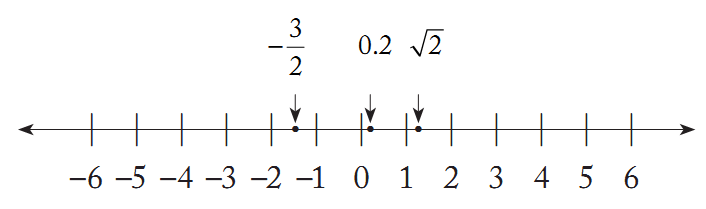
\includegraphics{../images/2022-05-31-01-38-22.png}

All real numbers (\(2, -7/5, \sqrt 3, \pi,\) etc.) are distinct points
on this number line.

When we extend the number system to include imaginary numbers (\(i\)),
we need to add another dimension to represent \emph{all complex
numbers.}

The \textbf{Complex Number Plane} is the visual representation of the
set of all Complex Numbers, where the x-axis represents \emph{real
numbers} and the y-axis represents \emph{imaginary numbers}

\begin{figure}
\centering
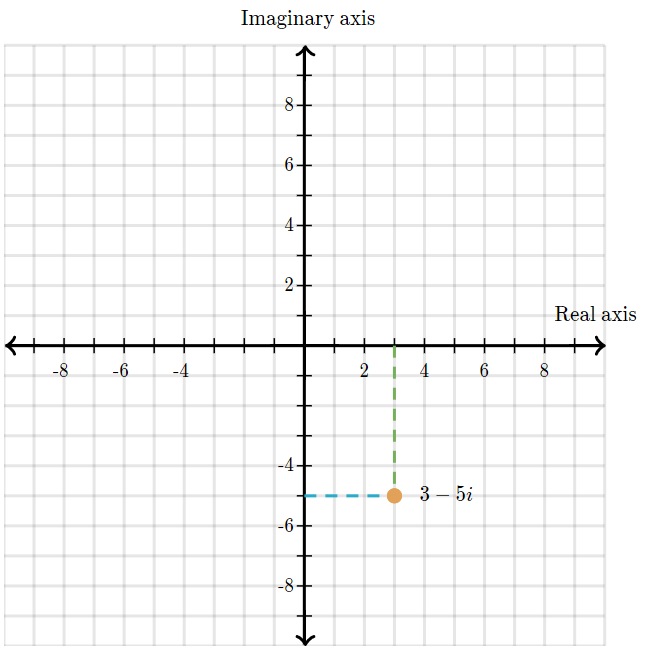
\includegraphics[width=4.6875in,height=\textheight]{../images/2022-05-31-01-34-44.png}
\caption{The Complex Number Plane}
\end{figure}

Each point on this plane represents a specific complex number.

Conversely, all complex numbers (\(3+i, \frac{-3}{2}+i\sqrt2, 57,\)
etc.) are represented by a point on the plane.

\begin{quote}
For any complex number, the modulus and conjugate can be visualised on
the complex plane.

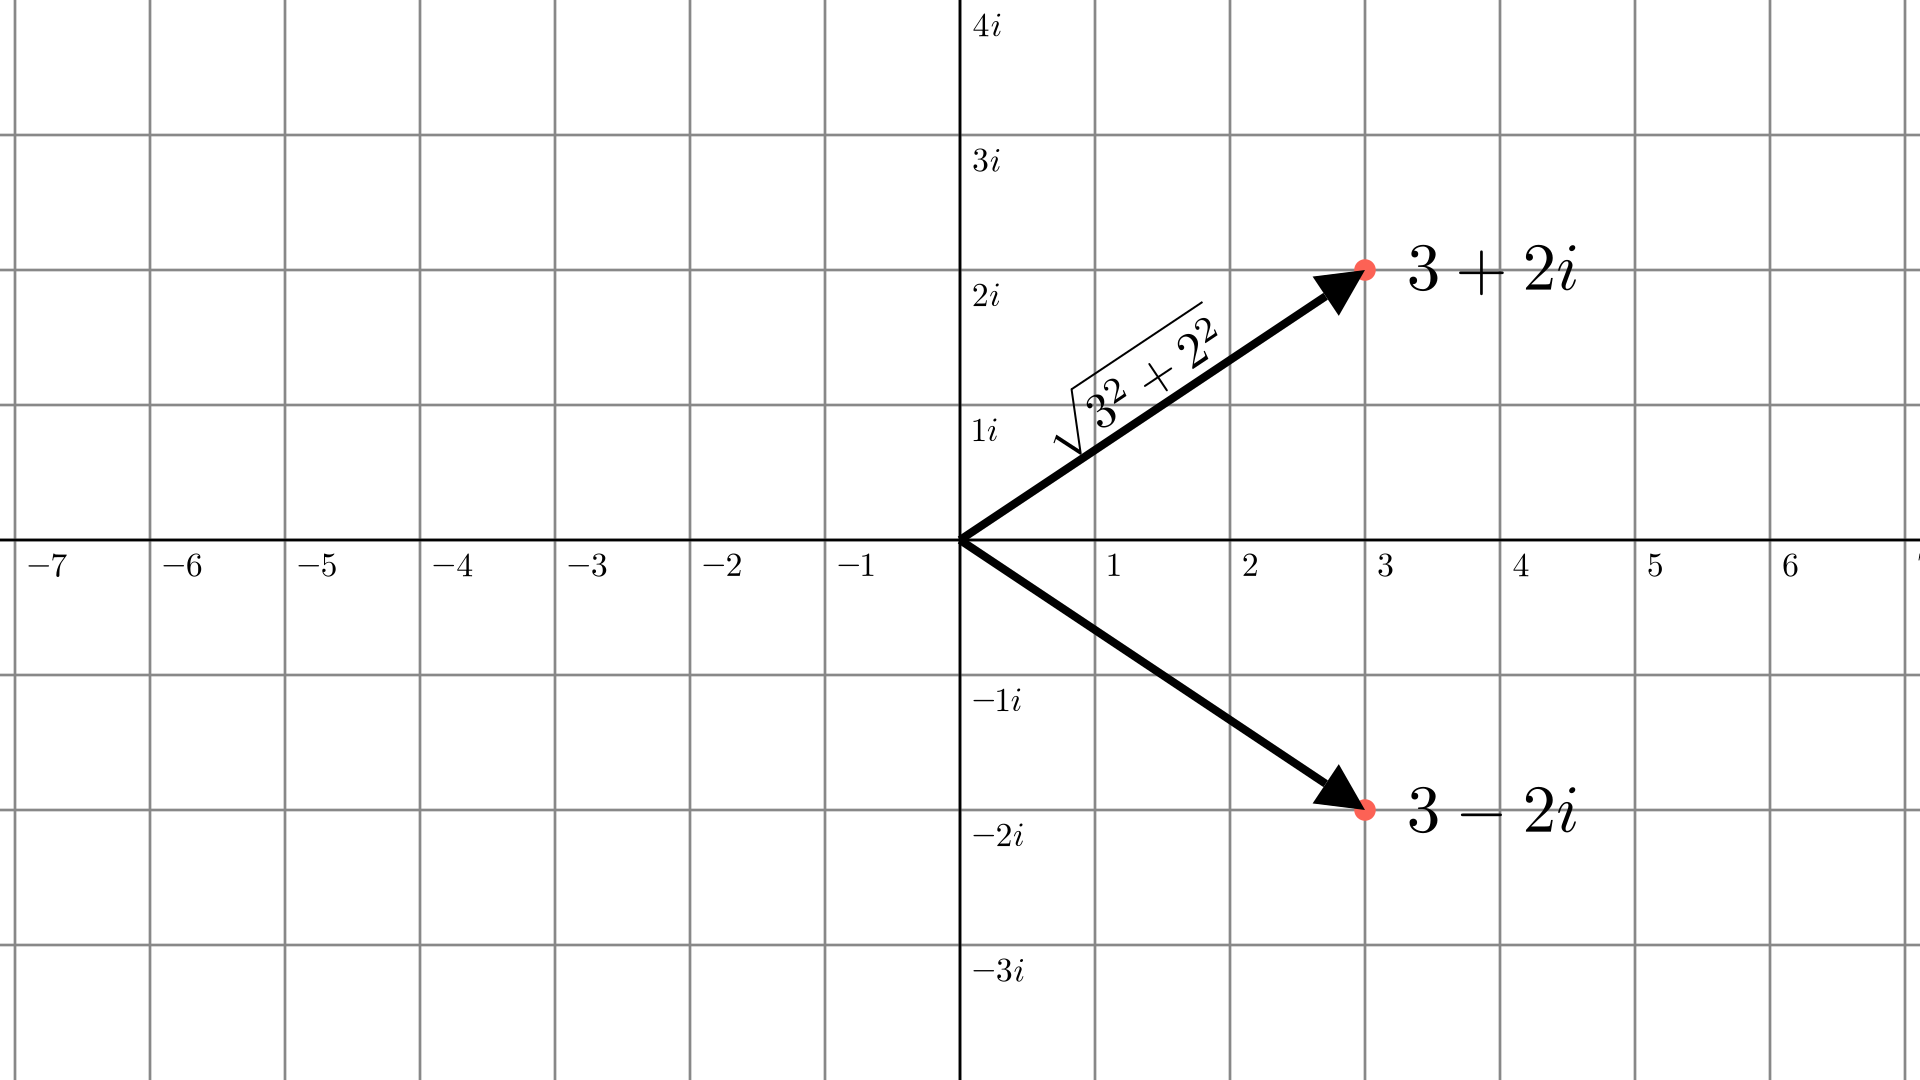
\includegraphics{../images/2022-05-31-15-27-09.png} The modulus of the
number is the distance of the point from the origin \(0\). The conjugate
of the number is the mirror image of the number on the Real axis.
\end{quote}

\hypertarget{cartesian-and-polar-coordinates}{%
\section{Cartesian and Polar
Coordinates}\label{cartesian-and-polar-coordinates}}

In the \textbf{Cartesian Coordinate System}, we use two numbers - the
x-coordinate and y-coordinate to locate a point on the plane.

\begin{figure}
\centering
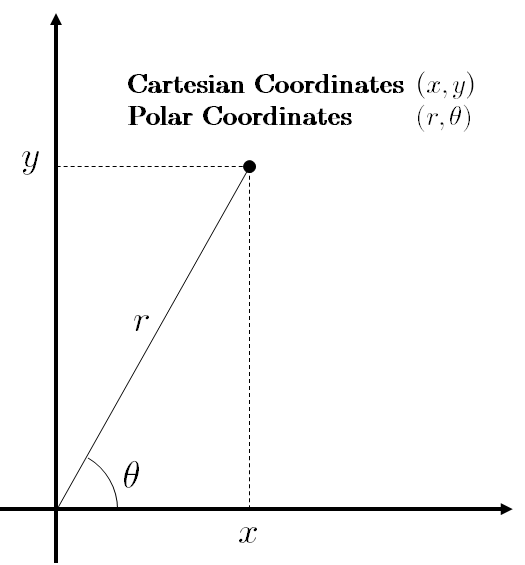
\includegraphics[width=3.64583in,height=\textheight]{../images/2022-05-31-17-15-48.png}
\caption{Cartesian and Polar Coordinates}
\end{figure}

Another system of Coordinates is the \textbf{Polar Coordinate System}.
Here, the two numbers used to represent a point in a plane are:

\[\text{Polar Coordinates: } (r,\theta)\]
\[r=\text{distance from origin}\]
\[\theta=\text{angle with horizontal axis}\]

\begin{quote}
For example, the point \(P(5, \pi/3)\) represents a point which is 5
units away from the origin, making a \(60\degree\) angle with the
x-axis.
\end{quote}

\hypertarget{complex-numbers-in-polar-form}{%
\subsection{Complex Numbers in Polar
Form}\label{complex-numbers-in-polar-form}}

When we represent complex numbers, we use the cartesian form \((x, y)\)
where \(x=\Re z\) and \(y=\Im z\). We can also use the polar system to
do so.

Let \(z\) be a complex number.

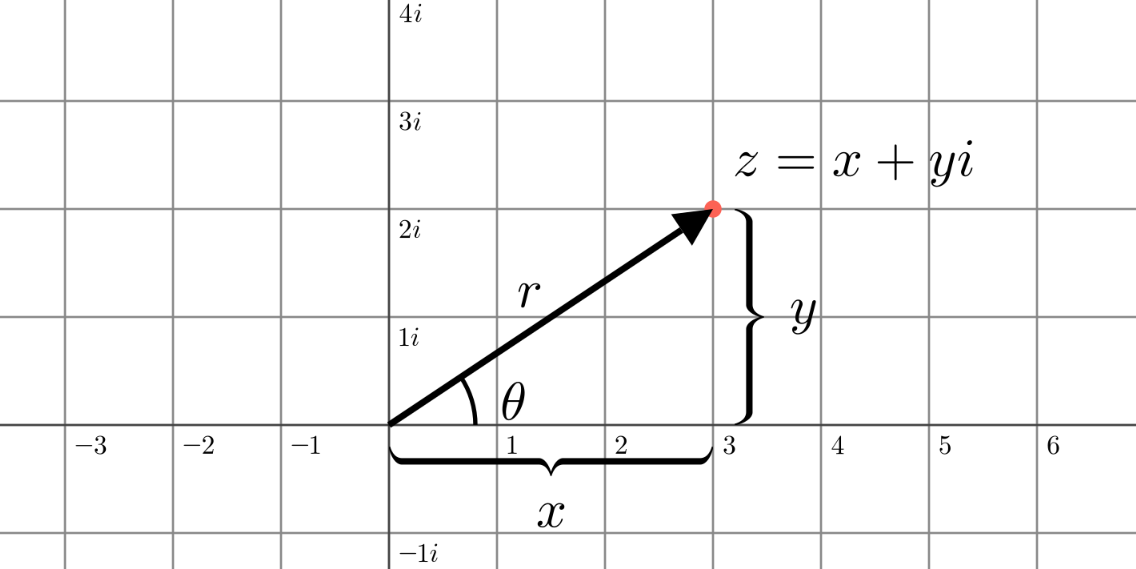
\includegraphics{../images/2022-05-31-19-12-30.png}

Here, we can calculate the x and y coordinates using
\textbf{trigonometry}.

\[x=r\cdot\cos\theta\] \[y=r\cdot\sin\theta\]

\[z=r\cos\theta+ir\sin\theta\] \[\boxed{z=r(\cos\theta+i\sin\theta)}\]
\[\ \tag{$r=\sqrt{x^2+y^2}=|z|$}\]

This is known as the Polar Representation of a Complex Number.

Here, \(\theta\) is known as the \textbf{argument} of \(z\).

\begin{quote}
There will be multiple values of \(\theta\) which satisfy the sin and
cos. By convention, we use the value \(-\pi<\theta\le\pi\)
\end{quote}

\begin{quote}
\textbf{Example} Find modulus and argument of \(1-i\). Also convert it
to the polar form.

\[z=1-i\] \[r=|z|=\sqrt{1^2+(-1)^2}\] \[\boxed{r=\sqrt2}\]
\[\cos\theta=\frac{\Re z}r=\frac1r=\frac1{\sqrt2}\]
\[\sin\theta=\frac{\Im z}r=\frac{-1}r=\frac{-1}{\sqrt2}\] sin is \(-\)ve
and cos is +ve \(\implies\) Angle in Quadrant IV
\[\boxed{\theta = \frac{-\pi}{4}}\] Polar Form:
\[\boxed{z=\sqrt2\left(\cos\frac{-\pi}4+i\sin\frac{-\pi}4\right)}\]
\end{quote}

\end{document}